\section{How FIDO2 Works}
This section offers a quick introduction into the FIDO2 ecosystem.
FIDO2 provides an phishing-resistant, origin-bound public-key authentication by combining the W3C WebAuthn API (browser/platform) with the FIDO Alliance CTAP protocol.

\subsection{Core Roles}
\begin{enumerate}
  \item \textbf{Relying Party (RP):} The application service that issues authentication challenges and stores each user's registered public key.
  \item \textbf{Client/Platform:} The browser or operating system that brokers WebAuthn requests and responses between the RP and the authenticator.
  \item \textbf{Authenticator:} A platform or roaming device that creates key pairs, enforces user presence/verification, and returns attested assertions.
\end{enumerate}

\subsection{Registration (makeCredential)}
\begin{enumerate}
  \item The RP provides options (challenge, RP ID, user handle, algorithm preferences) to the client.
  \item The authenticator creates a new key pair based on the RP ID, the private key remains within the authenticator, keeping it safe from attackers, the public key and attestation statement are returned.
  \item The RP verifies attestation and stores the credential public key.
\end{enumerate}

\subsection{Authentication (getAssertion)}
\begin{enumerate}
  \item The RP provides options (challenge, RP ID, and an allow list if applicable).
  \item The authenticator enforces user presence/verification, then signs the challenge together with the RP ID hash, authenticator flags, and a signature counter.
  \item The RP verifies origin, RP ID, signature, and counter before completing authentication.
\end{enumerate}

\subsection{Security Properties}
\begin{itemize}
    \item Origin binding (via RP ID and client data) mitigates phishing and relay.
    \item Non-exportable keys reduce the impact of server-side compromise.
    \item Attestation enables enforcement of device-class policy, lower class untrusted devices can be blocked.
\end{itemize}

\begin{figure}[htbp]
\centering
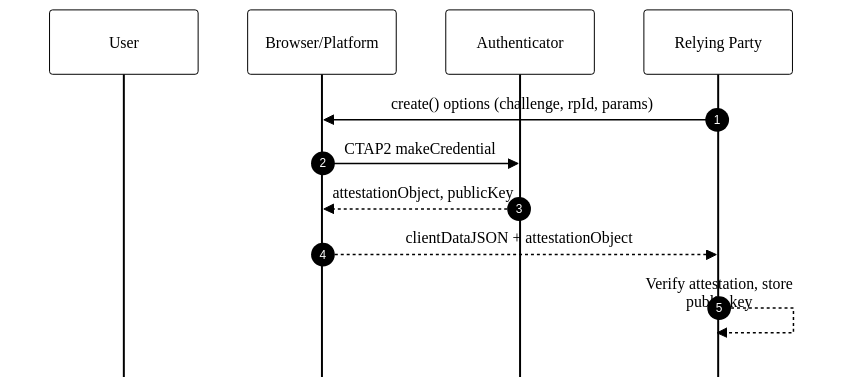
\includegraphics[width=\columnwidth]{resources/images/registration.png}
\caption{Registration sequence}
\end{figure}

\begin{figure}[htbp]
\centering
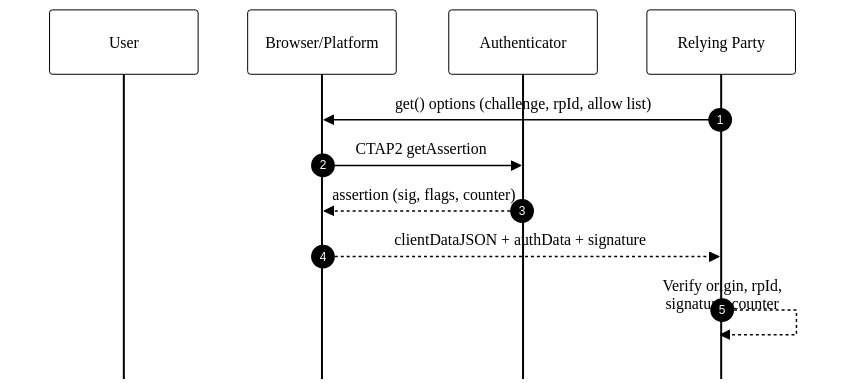
\includegraphics[width=\columnwidth]{resources/images/authentication.png}
\caption{Authentication sequence}
\end{figure}


\subsection{Real-World example}
This example tries to convey how Android devices keep the data secure working with the FIDO2 ecosystem.
On Android, passkeys and cryptographic keys are managed through Credential Manager and the Android Keystore. Where available, StrongBox places KeyMint in a discrete secure element so that keys are generated and stored within a dedicated secure processor rather than solely in the TEE. Private key material is non-exportable and invocable only via Keystore operations under enforced user-authentication and policy.

\subsubsection{StrongBox isolation}
StrongBox uses KeyMint in a separate secure chip. This chip has its own CPU,RAM and secure storage, completely isolating it from the mobile device, thus making it virtually impossible for bad-actors to access the private key stored here. I enables hardware attestation so servers can verify that keys are hardware-backed on a genuine device.

\subsubsection{Illustrative Flow}
\begin{itemize}
  \item The registration process begins through the Credential Manager (WebAuthn).
  \item The Keystore requests a hardware-backed key; on devices with StrongBox, the key pair is generated within the StrongBox KeyMint and marked as non-exportable.
  \item The public key and attestation chain are returned. The RP may verify the attestation to confirm hardware-backed security.
  \item During authentication, StrongBox performs the signature after local user verification; the private key never leaves the secure processor.
\end{itemize}
\begin{figure}[htbp]
\centering
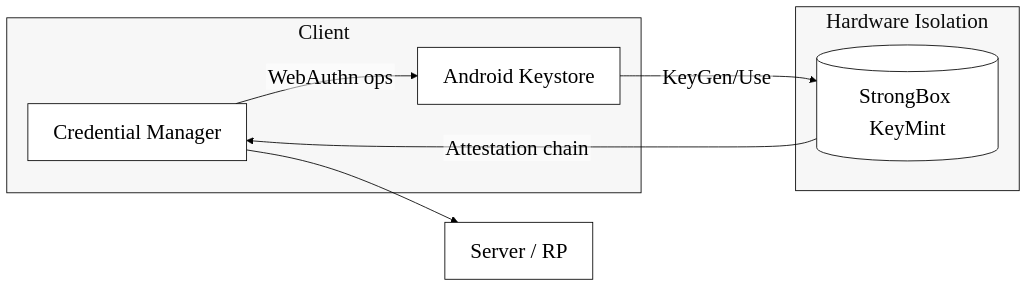
\includegraphics[width=\columnwidth]{resources/images/android_strongbox_flow.png}
\caption{Android StrongBox flow}
\end{figure}
